\section{Zielsetzung}
In diesem Versuch soll die Dichte, Schichtdicke und Rauigkeit einer Grenzfläche mittels einer Röntgenreflexionsmessung ermittelt werden.
Als Probe dient hierbei eine Polystyrolschicht, welche auf einem Silizium-Wafer aufgetragen ist und mit Hilfe eines Oberflächendiffraktometers der Firma Bruker-AXS untersucht werden soll.

\section{Theorie}
Die Wellenlänge der in Röntgenreflexionsversuchen verwendeten Strahlung liegt zwischen $\lambda = \SI{0,1}{\angstrom}$ und $\lambda = \SI{10}{\angstrom}$.
Röntgenstrahlen besitzen einen Brechungsindex der Form
\begin{equation}
    n=1-\delta + i \beta \, .
\end{equation}
Wobei $\delta = \frac{\lambda^2}{2\pi}r_e\rho > 0$ eine kleine Korrektur der Größenordnung $10^{-6}$ darstellt und $\beta = \frac{\lambda}{4\pi}\mu \approx 10^{-7}$ (für Röntgenstrahlung der Energie $E=\SI{8}{\keV}$) die Absorption beschreibt.
Die Tatsache, dass der Realteil des Brechungsindex kleiner als $1$ ist, ermöglicht das Auftreten von äußerer Totalreflexion, welche im folgenden Abschnitt genauer erläutert wird.

\subsection*{Röntgenreflektivität an glatten Grenzflächen}
Trifft eine elektromagnetische Welle in einem Medium mit dem Brechungsindex $n_1$ auf eine Grenzfläche zu einem Medium mit dem Brechungsindex $n_2$, so wird der Zusammenhang zwischen dem Winkel $\alpha_1$ der einfallenden Welle und dem Winkel $\alpha_2$ der transmittierten Welle durch das \textit{Snellius'sche Brechungsgesetz}
\begin{equation}
    \frac{\cos{\alpha_1}}{\cos{\alpha_2}}=\frac{n_2}{n_1}
\end{equation}
beschrieben.
Da für Röntgenstrahlung $\operatorname{Re}(n_2)<1$ ist, gilt stets $\alpha_2 < \alpha_1$.
Somit existiert ein kritischer Winkel $\alpha_1 = \alpha_c$ bei welchen $\alpha_2=0$ ist und es somit zur Totalreflexion der Welle kommt.
Unter Vernachlässigung der Absorption liegt dieser kritische Winkel bei 
\begin{equation}
    \alpha_c = \sqrt{2\delta} = \lambda \sqrt{\frac{r_e \rho}{\pi}}\, .
\end{equation}
Hierbei ist $\rho$ die Dichte des Materials und $r_e$ der klassische Elektronenradius.
Die Brechung einer elektromagnetischen Welle und die verwendeten Parameter sind in Abbildung \ref{fig:tfig1} dargestellt.
\begin{figure}[H]
\centering
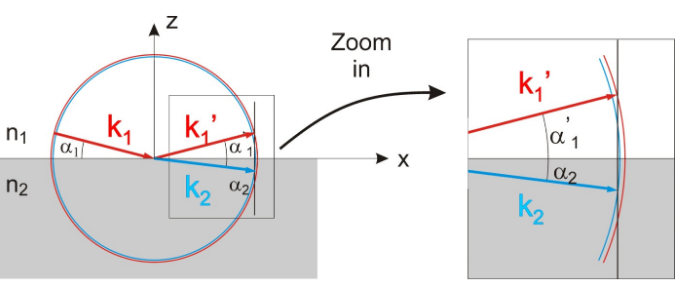
\includegraphics[width=0.8\linewidth]{figures/Reflexion}
\caption{Brechung einer elektromagnetischen Welle an einem optisch dünneren Medium. 
Der Einfallswinkel der Welle entspricht dem Ausfallswinkel der reflektierten Welle. 
Der Winkel $\alpha_2$ der transmittierten Welle ist stets kleiner als der Winkel $\alpha_1$, sodass es ab einem kritischen Winkel $\alpha_1 = \alpha_c$ zu Totalreflexion kommt \cite{XSR}.}
\label{fig:tfig1}
\end{figure}

Die \textit{fresnelschen Formeln} beschreiben den Reflexions- und Transmissionskoeffizient einer elektromagnetischen Welle an einer ebenen Grenzfläche.
Hierbei wird im Allgemeinen zwischen t- und s-polarisiertem Anteil der Welle unterschieden.
Im Falle von Röntgenstrahlung ist dieser Unterschied jedoch vernachlässigbar, sodass für den Reflexions- und Transmissionskoeffizient
\begin{align}
    r &= \frac{k_{i,z}-k_{t,z}}{k_{i,z}+k_{t,z}} = \frac{n_1\cos{\alpha_1}-n_2\cos{\alpha_2}}{n_1 \cos{\alpha_1}+n_2\cos{\alpha_2}}\\
    t &= \frac{2k_{i,z}}{k_{i,z}+k_{t,z}} = \frac{2 n_1\cos{\alpha_1}}{n_1 \cos{\alpha_1}+n_2\cos{\alpha_2}}
\end{align}
gilt.
Hierbei gilt $k_{i,z} = k \sin{\alpha_1}$ und $k_{t,z}= k\sqrt{n^2-\cos^2 \alpha_1}$.
Unter der Annahme, dass ${\alpha_1 > 3\alpha_c}$ gilt, beträgt die Fresnelreflektivität $R_\text{F}=|r|^2$ für Röntgenstrahlen näherungsweise
\begin{equation}
    R_\text{F}=\left(\frac{\alpha_c}{2\alpha_1}\right)^4\, . \label{eq:Reflektivitat}
\end{equation}
Abbildung \ref{fig:tfig2} zeigt die Reflektivität in Abhängigkeit des Einfallswinkels $\alpha_1$ am Beispiel von Silizium.
Wie die Formel \eqref{eq:Reflektivitat} erwarten lässt, ist eine starke Abnahme der Reflektivität für große Einfallswinkel zu beobachten.
\begin{figure}[H]
\centering
\includegraphics[width=0.6\linewidth]{figures/Reflektivität}
\caption{Reflektivität von Silizium in Abhängigkeit des Einfallswinkels $\alpha_1$ \cite{XSR}.}
\label{fig:tfig2}
\end{figure}

\subsection*{Röntgenreflektivität an mehreren Schichten}
Besteht das Medium aus mehreren Schichten so kommt es an jeder Schicht zu dem im vorherigen Kapitel beschriebenen Brechungsprozess.
Die reflektierten Wellen überlagern sich, sodass es je nach Einfallswinkel zu destruktiver und konstruktiver Interferenz kommt.
Abbildung \ref{fig:tfig3} zeigt die dadurch entstehende Oszillation der Reflektivität, welche auch \textit{Kiessig-Oszillation} genannt wird.
\begin{figure}[H]
\centering
\includegraphics[width=0.7\linewidth]{figures/Reflektivität2}
\caption{Reflektivität einer $\SI{800}{\angstrom}$ dicken Polystyrolschicht auf Silizium in Abhängigkeit des Einfallswinkels $\alpha_1$ für $\lambda = \SI{1,54}{\angstrom}$.
Die gestrichelte Linie zeigt die Reflektivität von Silizium nach Formel \eqref{eq:Reflektivitat} \cite{skript}.}
\label{fig:tfig3}
\end{figure}
Zu destruktiver Interferenz kommt es genau dann wenn der Gangunterschied der sich überlagernden Wellen ein ungerades Vielfaches der halben Wellenlänge beträgt.
So erlaubt die Lage der Oszillationsminima Rückschlüsse auf die Schichtdicke des Materials, welche demnach
\begin{equation}
    d = \frac{2\pi}{\Delta q_z}\approx \frac{\lambda}{2\Delta \alpha_1}
\end{equation}
beträgt.
Hier entspricht $q_z=2k\sin{\alpha_1}$ der z-Komponente des Wellenvektorübertrags und $\Delta q_z$ bzw $\Delta \alpha_1$ jeweils der Differenz dieser Größen an den Minima.

Die Reflektivität von Mehrschichtsystemen kann mit Hilfe des \textit{Parratt-Algorithmus} rekursiv bestimmt werden.
Hierzu kann aufgrund der geringen Eindringtiefe von Röntgenstrahlung angenommen werden, dass die unterste Schicht unendlich dick ist und es somit an dieser zu keiner weiteren Reflexion kommt.
Wie in Abbildung \ref{fig:tfig4} dargestellt, kommt es an jeder Grenzfläche der Dicke $d_j = z_{j-1}-z_j$ mit dem Brechungsindex $n_j=1-\delta_j+i\beta_j$ zu einer Reflexion mit der Fresnelreflektivität $r_{j, j+1}=\frac{k_{z,j}-k_{z,j+1}}{k_{z,j}+k_{z,j+1}}$.
Hierbei entspricht $k_{z,j}= k\sqrt{n_j^2-\cos^2(\alpha_1)}$ der z-Komponente des Wellenvektors in der $j$-ten Schicht.
\begin{figure}[H]
\centering
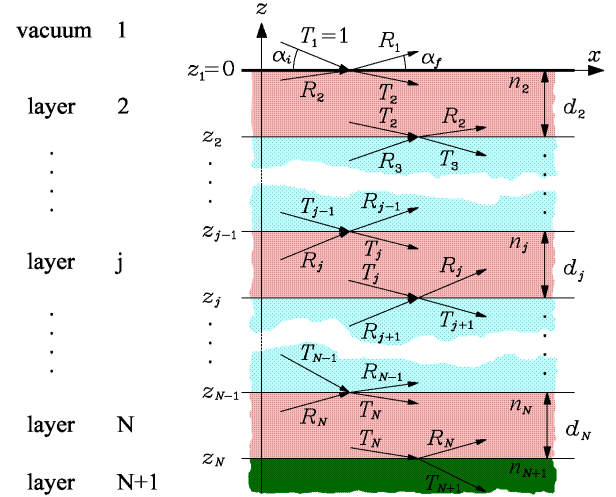
\includegraphics[width=0.7\linewidth]{figures/Parratt}
\caption{Darstellung eines Mehrschichtsystems mit $N+1$ Schichten und $N$ Grenzflächen.
Für jede Schicht sind die Reflexions- und Transmissionskomponenten zu sehen.
Die $(N+1)$-te Schicht wird als unendlich Dick angenommen, sodass keine weitere Reflexion auftritt \cite{skript}.}
\label{fig:tfig4}
\end{figure}
Das Verhältnis der Amplituden der reflektierten und transmittierten Welle an der $j$-ten Grenzfläche entspricht nach dem Parratt Algorithmus
\begin{equation}
    X_j = \frac{R_j}{T_j}=\exp(-2ik_{z,j}z_j)\frac{r_{j, j+1}+X_{j+1}\exp(2ik_{z,j+1}z_j)}{1+r_{j,j+1}X_{j+1}\exp(2ik_{z,j+1}z_j)}\, .
\end{equation}

\subsection*{Röntgenreflektivität an rauen Grenzflächen}
In der Realität besitzen Grenzflächen immer eine endliche Rauigkeit, sodass die gemessene Reflektivität geringer ist als die Fresnelreflektivität.
Die Rauigkeit wird durch die Einführung der modifizierten Fresnelkoeffizienten
\begin{align}
    \tilde{r}_{j, j+1} &= r_{j,j+1}\exp\left(-2k_{z,j}k_{z,j+1}\sigma_j^2\right)\\
    \tilde{t}_{j, j+1} &= t_{j,j+1}\exp\left(\frac{1}{2}(k_{z,j}-k_{z,j+1})^2\sigma_j^2\right )\\
\end{align}
berücksichtigt. Dabei bezeichnet $\sigma_j$ die Rauigkeit der $j$-ten Schicht.

\vspace{20pt}
\begin{figure}[H]
\begin{minipage}[t]{0.54\textwidth}
\vspace{-110pt}
\subsection*{Geometriefaktor und Geometriewinkel}
Wie in Abbildung \ref{fig:tfig5} zu sehen ist, trifft erst ab einem genügend großen Einfallswinkel $\alpha_1 > \alpha_g$ der gesamte Strahl auf die Oberfläche und wird reflektiert.
Da in diesem Versuch sehr kleinen Winkeln $\alpha_1$ verwendet werden, wird dieser Intensitätsverlust durch den sogenannten \textit{Geometriefaktor}
\begin{equation}
    G = \frac{D\sin{\alpha_1}}{d_0} \qquad \text{mit} \qquad \alpha_1 < \alpha_g
\end{equation}
\end{minipage}
\begin{minipage}[t]{0.44\textwidth}
\centering
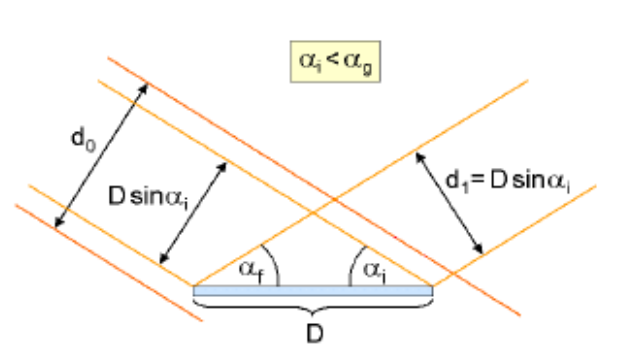
\includegraphics[width=1\linewidth]{figures/Geometriefaktor}
\vspace{-20pt}
\caption{Strahlenverlauf für $\alpha_1<\alpha_G$ \cite{skript}}
\label{fig:tfig5}
\end{minipage}
\end{figure}
\vspace{-10pt}
berücksichtigt. Hierbei stellt $D$ den Probendurchmesser und $d_0$ den Durchmesser des Strahls dar.

